% ===================================================================
%                   Presentación con Latex Beamer
% ===================================================================
\documentclass[9pt,xcolor=svgnames]{beamer}
%\documentclass[handout,xcolor=svgnames]{beamer} %Version imprimible
% -------------------------------------------------------------------
% Paquetes personalizados
\usepackage{../paquetes}
\usepackage{../colores}
\usepackage{../info}
\usepackage{../modo}
% -------------------------------------------------------------------

% Comienza el documento
\begin{document}
% Tikz -> Imágenes
\tikzstyle{every picture}+=[remember picture]
% Entorno matemático
\everymath{\displaystyle}
% -------------------------------------------------------------------
\subtitle{El avance del proyecto}
% -------------------------------------------------------------------
% Fondo blanco: primera página
% ------------------------------------------------------------------

\beamersetaveragebackground{white}

\begin{frame}
 \thispagestyle{empty}
 
 \animate<2-3> 
 \begin{figure}[t]
  \centering
  \includegraphics<1>[scale=0.7]{../Imagenes/logo_1.pdf}
  \includegraphics<2>[scale=0.7]{../Imagenes/logo_2.pdf}
  \includegraphics<3>[scale=0.7]{../Imagenes/logo_3.pdf}
  \includegraphics<4>[scale=0.7]{../Imagenes/logo_4.pdf}
 \end{figure}
\end{frame}


% -------------------------------------------------------------------
% Fondo para el resto del documento
\setbeamertemplate{background}{

\includegraphics[width=\paperwidth,height=\paperheight]
{../Imagenes/fondo.pdf}
}
% -------------------------------------------------------------------


% Continuación:
% Transparencia de Inicio -> Título
\begin{frame}
 \titlepage
\end{frame}

\normalsize

% Transparencia de índice
\begin{frame}{Índice} 
 \transboxin
 \tableofcontents
\end{frame}
  
  
 \section{Estado del proyecto}
 
  \subsection{Actualización de la planificación}
  
  \begin{frame}{Diagrama de Gannt}
   \transdissolve
   
   \begin{figure}[t]
    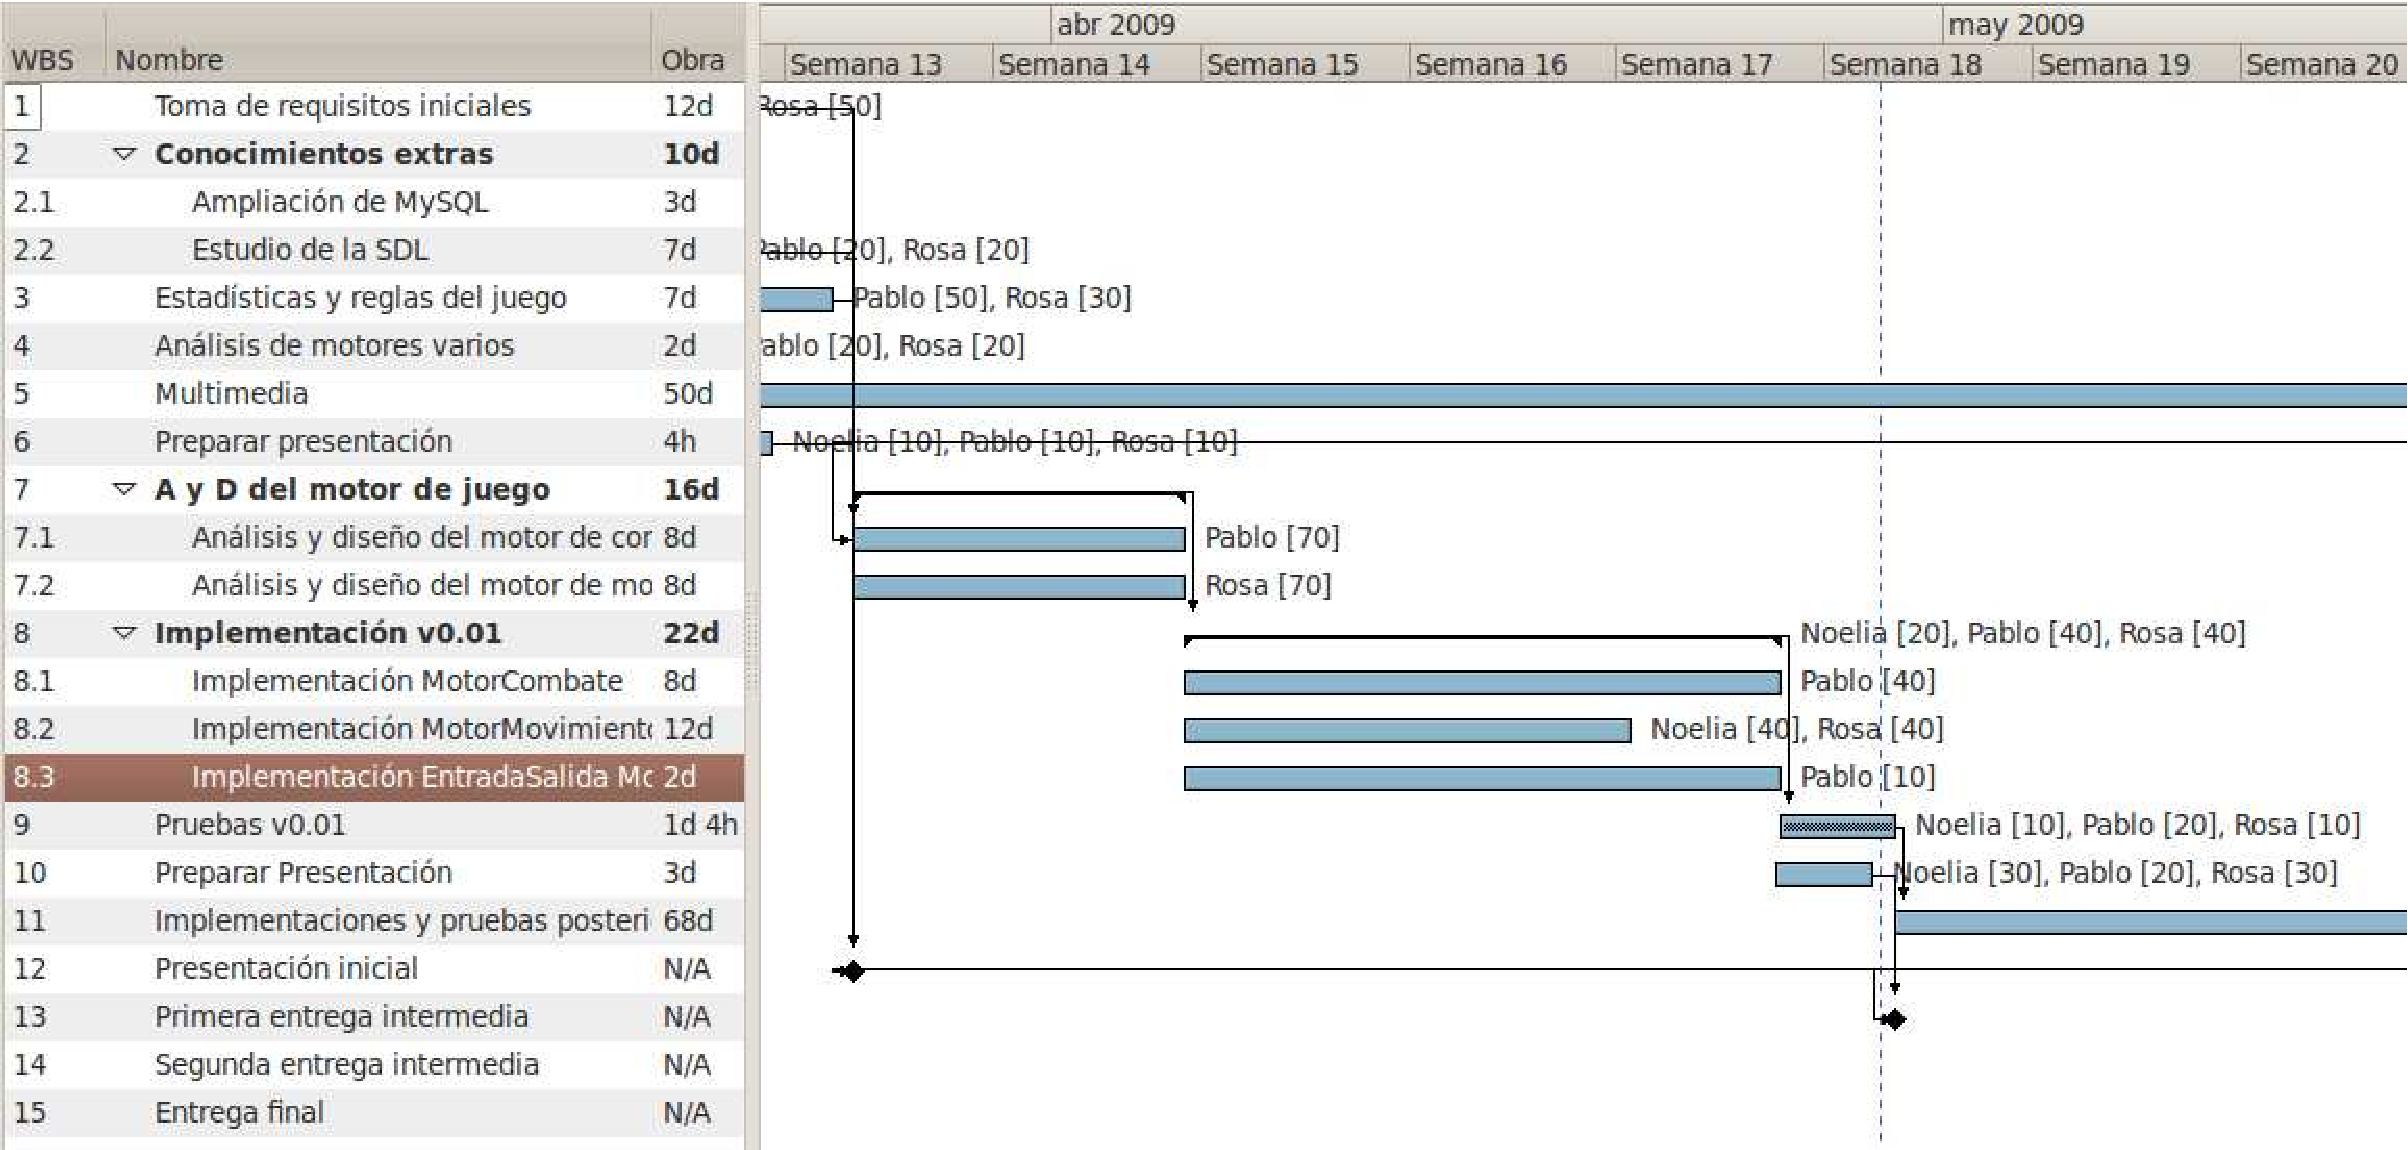
\includegraphics[scale=0.27]{./Imagenes/gannt.pdf}
   \end{figure}
   
  \end{frame}
  
  
  \begin{frame}{Asignación de Recursos}
   
   Actualmente centrándonos en la implementación:
   
   \begin{block}{Motor de combate}
    \begin{description}
     \item[Desarrollador principal:] Pablo.
     \item[Estado actual:] versión de prueba de combate sin gráficos.
     \item[A completar:] parte gráfica.
    \end{description}
   \end{block}

   \begin{block}{Motor de movimiento}
    \begin{description}
     \item[Desarrolladoras principales:] Rosa y Noelia.
     \item[Estado actual:] finalizados los elementos necesarios para el 
		movimiento básico y la visualización de gráficos, así
		como los de gestión de eventos externos. 
     \item[A completar:] sección correspondiente a los menús y a la
	   carga/guardado de niveles.
    \end{description}
   \end{block}
    
  \end{frame}
   
   
   
   \subsection{Modificaciones sufridas por el proyecto}
   
   \begin{frame}{Modificaciones y justificaciones}
    
    \begin{block}{Utilización de ficheros XML}
     Para guardar la configuración del juego, así como para ``diseñar''
     y mantener en un formato simple la distribución de los diferentes
     niveles de juego.\\
     \vspace*{0.5cm}
     
     Potenciamos así la posibilidad de que se incrementen los niveles del
     juego.
    \end{block}
    
   \end{frame}
   
   
   
 \section{Calidad del proyecto software}
 
  \subsection{Ingeniería del software}
  
  \begin{frame}{Modelo incremental aplicado al proyecto}   
   \transdissolve
   
   Basándonos en nuestra experiencia, está resultando bastante apropiado.
   
   \begin{itemize}
    \item Modificar conforme se observan posibles mejoras.
    \item No abarcar demasiado para una versión primitiva. Poco a poco.
   \end{itemize}
   
  \end{frame}
  
  
  \subsection{Ejemplo: Análisis y diseño del motor gráfico}
  
  \begin{frame}{Diagrama de Casos de Uso}

   \begin{figure}[t]
    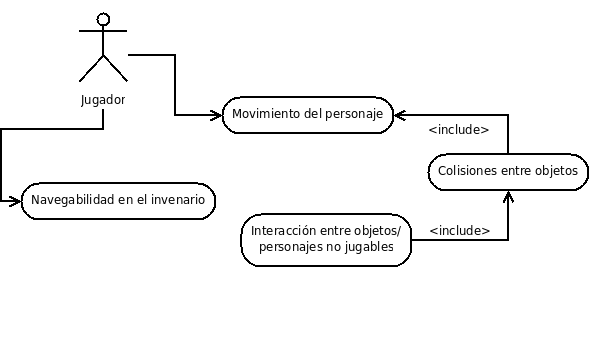
\includegraphics[scale=0.4]{./Imagenes/Diagrama_Casos_Uso.png}
   \end{figure}
  \end{frame}
  
  
  
  \begin{frame}{Ejemplo: Descripción Caso de Uso}
   
   \textbf{Caso de Uso:} \textsc{Movimiento del personaje}
   
   \begin{description}
    \item[Caso de Uso:] Movimiento del personaje.
    \item[Descripción:] El jugador podrá realizar cuatro tipos de
	  movimientos con el personaje principal: trasladar el personaje
	  hacia arriba, hacia abajo, hacia la derecha o hacia la
	  izquierda del mapa.
    \item[Actores:] Usuario o jugador del videojuego.
    \item[Precond:] El videojuego está iniciado y está
	  cargado todo el motor de movimiento sin errores.
    \item[Postcond:] Ninguna.
    \item[Escenario principal:] $\quad$	  
	       \begin{enumerate}
		\item El jugador pulsa la tecla 'up' del teclado.
		\item El sistema mueve el personaje del juego hacia arriba
		      del mapa.
		\item El jugador colisiona con un objeto. \textbf{Include:
		      Colisiones entre objetos.}
	       \end{enumerate}
   \end{description}
  \end{frame}
  
  
  \begin{frame}{Ejemplo: Descripción Caso de Uso}

   \begin{description}    
    \item[Escenarios alternativos o de error:] $\quad$	       
	       \begin{itemize}
		\item El jugador pulsa la tecla 'down' del teclado.
		      El sistema mueve el personaje del juego hacia
		      abajo del mapa.
		\item El jugador pulsa la tecla 'left' del teclado.
		      El sistema mueve el personaje del juego
		      hacia la izquierda del mapa.
		\item El jugador pulsa la tecla 'right' del teclado.
		      El sistema mueve el personaje del juego
		      hacia la derecha del mapa.
		\item El personaje se encuentra en un borde de la
		      pantalla y quiere avanzar (cualquier dirección).
		      \begin{enumerate}
		       \item El sistema comprueba que existe más mapa
			     fuera de la pantalla y hace que el
			     personaje acceda a esa porción del mapa.
		       \item El sistema comprueba que no existe más mapa
			     para visualizar en dicha dirección y deja
			     al personaje en la misma posición.
		      \end{enumerate}
	       \end{itemize}
   \end{description} 
  \end{frame}
  
  
  \begin{frame}{Diagrama de Casos de Uso}
   \begin{figure}[t]
    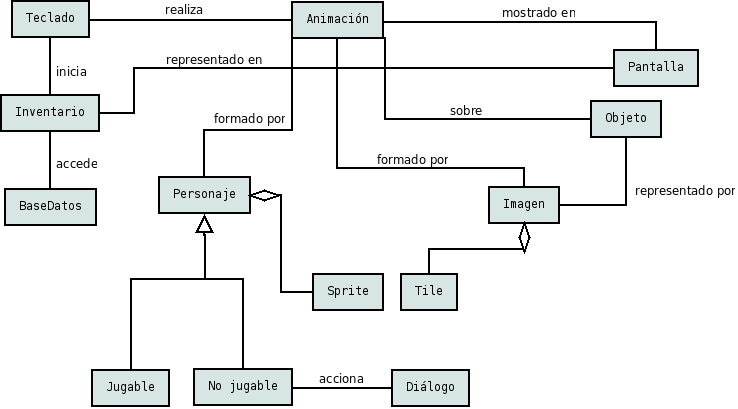
\includegraphics[scale=0.34]{./Imagenes/Diagrama_conceptual.png}
   \end{figure}
  \end{frame}
  
  
  
 \section{Resultados obtenidos}
 
  \subsection{Algoritmo general en pseudocódigo}

  \begin{frame}{Algoritmo}
   
   \begin{description}
    \item[1.] Se ejecuta el programa.
    \item[2.] Se cargan los ficheros de configuración.
    \item[3.] Se inicia el videojuego mostrando el menú principal.
	  
	       \begin{itemize}
		\item El jugador elige jugar.\\
		      Se muestra en pantalla las opciones de crear nuevo
		      juego o cargar uno existente.
		      
		      \begin{itemize}
		       \item El jugador crea un nuevo juego. \\
			     Se cargan los ficheros iniciales. \\
			     Se muestra una animación de la introducción
			     del juego.			     
		       \item El jugador elige  cargar un juego existente. \\
			     Se cargan los ficheros configurados
			     para el usuario.
		      \end{itemize}
	       \end{itemize}
   \end{description}
   
  \end{frame}

  \begin{frame}{Algoritmo}

   \begin{description}
    \item[4.] El usuario comienza a jugar (con el motor de movimiento).
    \item[5.] El jugador mueve el personaje.
	  
	  \begin{itemize}
	   \item El personaje se mueve sin ningún inconveniente.
	   \item El personaje no se puede mover (colisiona con un objeto).
	   \item El personaje no se puede mover, pero sí interactuar:	 
		 \begin{itemize}
		  \item Comienza un combate.		  
		  \item Interactúa con un objeto.
		  \item Dialoga con otro personaje.			
		 \end{itemize}
		 
	  \end{itemize}
   \end{description}

  \end{frame}
  
  
  \begin{frame}{Algoritmo}

   \begin{description}
    \item[5.1.] El jugador entra en el inventario.
	  
	  \begin{itemize}
	   \item Visualiza la pestaña contenedora del estado de los
		 personajes.
	   \item Visualiza la pestaña contenedora de los objetos que tiene el
		  grupo.
	   \item Visualiza la pestaña que contiene las opciones Guardar y
		 Salir.
	  
		 \begin{enumerate}
		  \item El usuario guarda el juego.\\
			El sistema guarda el estado del juego.
		  \item El usuario sale del juego.\\
			El sistema destruye la memoria dinámica
			utilizada y sale del programa.		  
		 \end{enumerate}
	  \end{itemize}
	  
    \item[6.] El jugador elige salir.
    \item[7.] El sistema sale del programa.	  
   \end{description}
  \end{frame}
    
    
  \subsection{Implementación}
  
  \begin{frame}{Clases ya implementadas}
   
    \begin{columns}
     
     \begin{column}{3cm}
      \begin{block}{Motor de combate}
       \begin{itemize}
	\item Atributos
	\item Atributos-base
	\item Combatiente
	\item Especial
	\item Grupo
	\item Habilidad
	\item Inventario
	\item Objeto      
       \end{itemize}
      \end{block}
     \end{column}
     
     \begin{column}{3cm}
      \begin{block}{Motor gráfico}
       \begin{itemize}
	\item Animación
	\item Evento
	\item Imagen
	\item Pantalla
	\item Personaje
	\item Sprite
	\item Tile
       \end{itemize}
      \end{block}
     \end{column}
     
    \end{columns}
  \end{frame}
  
  \begin{frame}{Para muestra...}
   
   No vamos a enseñar código, puesto que sería entrar demasiado en
   materia y requeriría demasiado tiempo.\\ 
   \vspace*{0.5cm}
   
   Resulta más efectivo y más entretenido ver como funciona.
   
  \end{frame}
  
  
  \subsection{Multimedia}

  
  \begin{frame}{Imágenes}

   Además de los sprites de movimiento, hemos seguido desarrollando y
   buscando más imágenes que nos puedan ser útiles.\\

   \begin{itemize}
    \item Iconos de origen propio.\\
	  A utilizar en algun menú\footnote{Todavía por considerar}.
	  
	  \begin{figure}[t]
	   
\includegraphics[scale=0.6]{./Imagenes/iconos.pdf}
	  \end{figure}
	  
   \end{itemize}

  \end{frame}

  
  \begin{frame}{Imágenes}
   
   \begin{itemize}
    \item Menú de inicio del juego\footnote{Lógicamente es el esquema
	  conceptual: lo que se ha diseñado son los elementos y el fondo
	  por separado.} de origen propio.
	  
	  \begin{figure}[t]
	   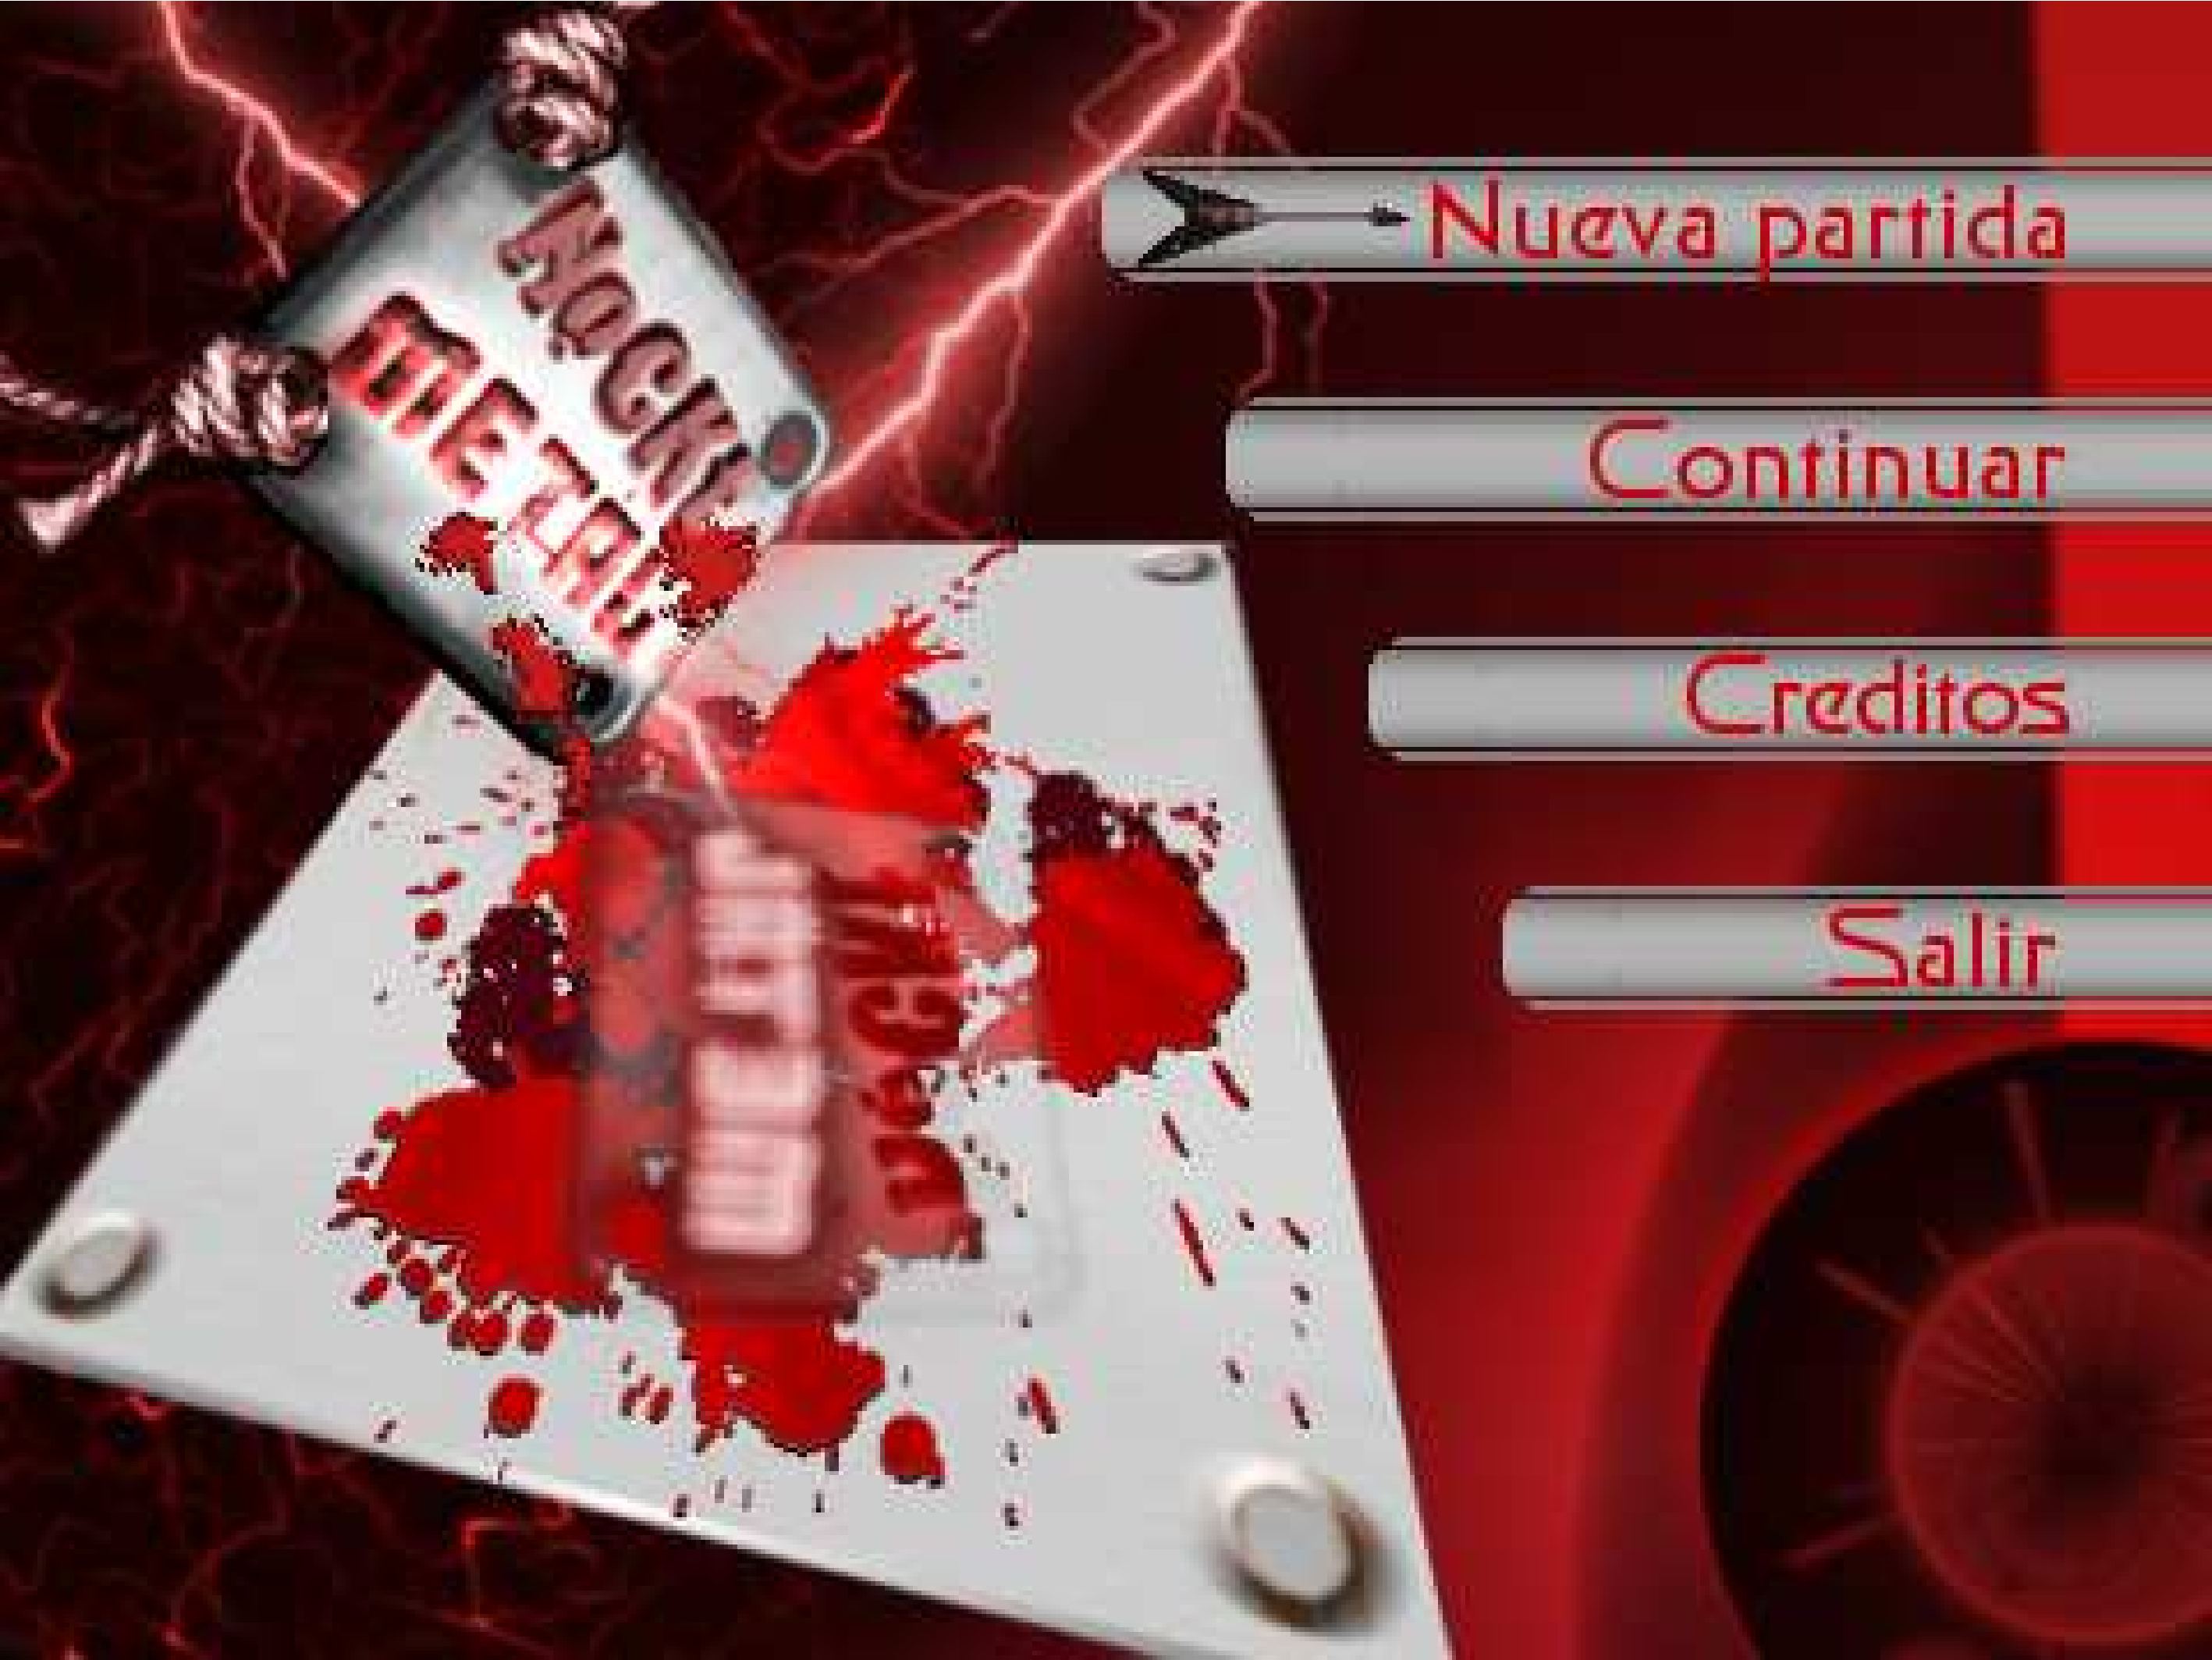
\includegraphics[scale=0.15]{./Imagenes/menu.pdf}
	  \end{figure}
   \end{itemize}
   
  \end{frame}
  
  
  
  \begin{frame}{Imágenes}
   
   \begin{itemize}
    \item Objetos varios incluidos en \textit{Battle for Wesnoth} bajo
	  GPLv3\\
	  \url{http://www.gnu.org/licenses/gpl-3.0.html}
	  
	  \begin{figure}[t]
	   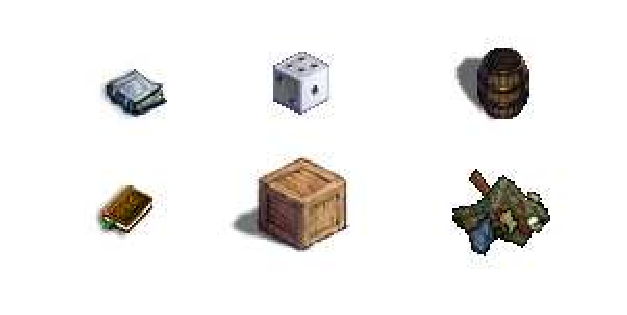
\includegraphics[scale=0.5]{./Imagenes/objetos.pdf}
	  \end{figure}
	  
   \end{itemize}
   
  \end{frame}
  
  
  
  \begin{frame}{Imágenes}
   
   \begin{itemize}	  
    \item Tiles varios, algunos de origen propio, otros incluidos en
	  \textit{Battle for Wesnoth} bajo GPLv3\\
	  \url{http://www.gnu.org/licenses/gpl-3.0.html}
	  
	  \begin{figure}[t]
	   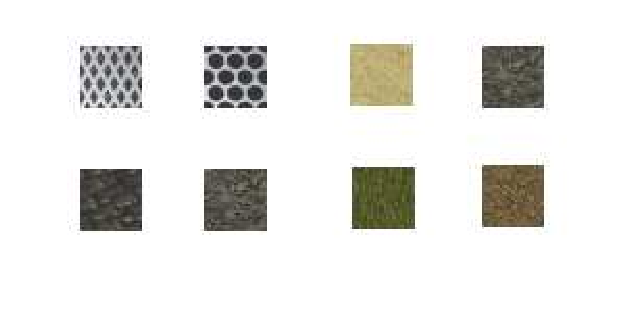
\includegraphics[scale=0.5]{./Imagenes/tiles.pdf}
	  \end{figure}
	  
   \end{itemize}
   
  \end{frame}
  
  
  \begin{frame}{Audio}
   \begin{itemize}
    \item \textit{The Slip} $\longrightarrow$ \textit{Nine Inch Nails}
	  bajo Creative Commons\\
	  \textsc{Attribution-Noncommercial-Share Alike 3.0}\\
	  \url{http://creativecommons.org/licenses/by-nc-sa/3.0/us/}\\
	  \vspace*{0.3cm}	  

    \item Efectos de sonido de \textit{Battle for Wesnoth} bajo GPLv3\\
	  \url{http://www.gnu.org/licenses/gpl-3.0.html}\\
	  \vspace*{0.3cm}
	  
    \item Posibilidad de incluir música variada (encuadrada bajo el
	  estilo metal) bajo Creative Commons.
	  \url{www.soundclick.com}\\
	  \url{www.jamendo.com}
   \end{itemize}
  \end{frame}
  
  
 \section{Metodología de trabajo}
 
  \subsection{SVN y forja}

  \begin{frame}{Trabajando en grupo}
   
   \begin{itemize}
    \item Actualmente llevamos más de 100 revisiones desde que se inició
	  el desarrollo en el repositorio de la forja.\\
	  \vspace*{0.3cm}

    \item Nos servimos de las listas de correo para informar de
	  actualizaciones o commits importantes.\\
	  Así nos aseguramos de que el resto del grupo tiene noticia de
	  la aparición o solución de un bug.\\
	  \vspace*{0.3cm}
	  
    \item Consenso en el estilo de programación, así como en la
	  utilización de unos parámetros fijos en la documentación de
	  Doxygen (como \textbf{@todo}).\\
	  \vspace*{0.3cm}

    \item Participación y colaboración con otros grupos.
   \end{itemize}
  \end{frame}
  
  
  \subsection{Elementos extras del proyecto}
  
  \begin{frame}{Elementos extras}
   \begin{itemize}
    \item Página web
    \item Documentación actualizada a diario
    \item Manual de usuario (enfocado al jugador principiante)
   \end{itemize}
  \end{frame}

 \section{Para terminar}
  
\scriptsize

 \begin{frame}{Esta presentación es libre}
  Copyright 2009 Noelia Sales Montes\\
  Parte del Proyecto NoCKt Metal\\
  \url{http://nocktmetal.forja.rediris.es/}
  
  \vspace*{0.3cm}
  
  Creative Commons Attribution License
  \url{http://creativecommons.org/licenses/by/2.0/}\\
  Creative Commons, 559 Nathan Abbott Way, Stanford, California 94305,
  USA.
  
  \vspace*{0.3cm}
  
  Este trabajo se publica bajo la siguiente licencia:\\
  Creative Commons Attribution License
  \url{http://creativecommons.org/licenses/by/3.0/}
  
  \vspace*{0.3cm}
  
  Usted es libre de:
  \begin{itemize}
   \item copiar, distribuir y comunicar públicamente la obra
   \item hacer obras derivadas
  \end{itemize}
  
  Bajo las condiciones siguientes:
  \begin{itemize}
   \item Reconocimiento. Debe reconocer los créditos de la obra de la
	 manera especificada por el autor o el licenciador (pero no de una
	 manera que sugiera que tiene su apoyo o apoyan el uso que hace de
	 su obra).
   \item Al reutilizar o distribuir la obra, tiene que dejar bien claro los
	 términos de la licencia de esta obra.
   \item Alguna de estas condiciones puede no aplicarse si se obtiene el
	 permiso del titular de los derechos de autor
   \item Nada en esta licencia menoscaba o restringe los derechos morales
	 del autor.
  \end{itemize}
 \end{frame}


  
\end{document}
 
